% !TEX root = ./main.tex
\chapter{Impacts of emissions spatial heterogeneity on gas-phase reactions}

This chapter investigates the impacts of pure gas phase emissions and associated chemical reactions on the production of ozone in the planetary boundary layer. The effect emissions spatial heterogeneity on ozone production is explored across numerous emissions scenarios with ranging emissions spatial heterogeneity. We find that for the most heterogeneous emissions case, ozone production is reduced in the mid-boundary layer by up to $\sim12\%$.

\section{Simulated emission scenarios}

\begin{figure}[h]
	\centering
	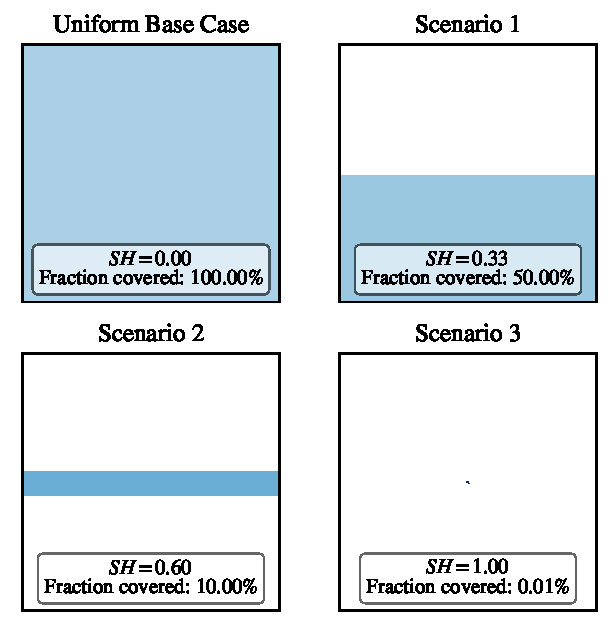
\includegraphics[width=.7\textwidth]{SH-scenarios-main-runs.pdf}
	\caption{Emissions scenarios for ozone production simulations. The spatial heterogeneity of each emission scenario is listed in the lower portion of each scenario alongside domain mean and variance.}
	\label{fig:ozone-emission-patterns}
\end{figure}

We conduct four simulations in total ranging in emissions spatial heterogeneity from $SH=0$ to $SH=1$ for precursor species responsible the production of ozone. Emissions scenarios are shown in Figure \ref{fig:ozone-emission-patterns}. The first simulation, named the uniform base case scenario, is characterized by uniform emissions of all compounds across the computational domain ground level. The uniform base case has a spatial heterogeneity equal to zero. This scenario represents the emissions across a single grid cell in a lower resolution model, such as a regional or global climate model, where emitted species are both uniform and dilute. Thus, results for simulations with higher emissions heterogeneity are compared against the uniform base case to quantify the structural uncertainty in ozone concentrations resulting from the assumption of uniform, dilute emissions characteristic of coarser resolved models that do not adequately resolve the true emissions spatial heterogeneity.  

Across the simulated emission scenarios, the area occupied by ground level emissions decreases up to a single grid cell in the case of emissions scenario 3. This scenario is meant to represent a highly localized emissions source and is the maximally heterogeneous case with $SH=1$. The total mass per unit time emitted across each scenario remains the same, thus the emission rate for high spatial heterogeneity cases must be scaled by the ratio between the area occupied by emissions in the uniform base case and the area emissions occupy in the corresponding emissions scenario. For example, the area of emissions in emissions scenario 3 is $0.01$ \si{km^2} while the area occupied by emissions in the uniform base case is  $100$ \si{km^2}, resulting in an emissions rate scaling factor of $100/0.01 = 10,000$. 

Each simulation was run for a total of 6 hours beginning at 9:00 AM LT and ending at 3:00 PM LT. The first hour of each simulation allows spin up and development of the PBL. Afterward, emissions occur at a constant rate for the remainder of each simulation.

\section{Results}


\subsection{Ozone cross sections}

In order to visualize the spatial heterogeneities present in ozone throughout each simulation, cross sections of ozone concentrations in the x-y plane were plotted for each emissions scenario. Cross sections were selected at a vertical level corresponding to the approximate middle of the PBL ($z\sim500$ \si{m}) and were plotted at regular, 2 hour intervals. 

Ozone cross section plots for the uniform base case are shown in Figure \ref{fig:o3-crosssec-ub}. Ozone concentrations are displayed as molar fractions in parts per billion by volume (ppbv). Throughout each snapshot, the distribution of ozone is shown to be nearly uniform with minimal concentration gradients. Ozone concentrations steadily increase throughout the course of the simulation, reaching in excess of 110 ppbv by $t=6$ h.

Ozone cross sections for emission scenarios 1--3 are shown in Figures \ref{fig:o3-crosssec-s1}--\ref{fig:o3-crosssec-s3}, respectively.

\begin{figure}[h]
    \centering
    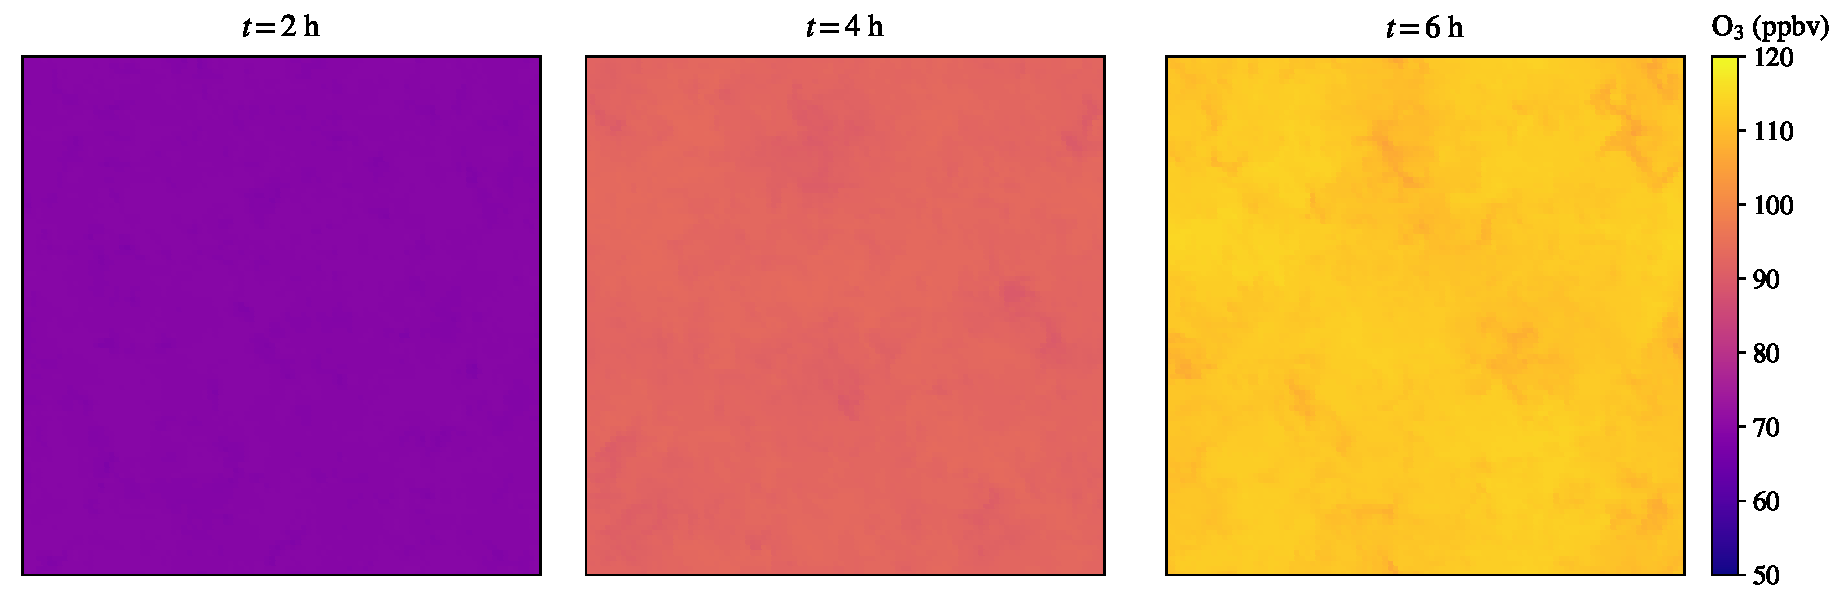
\includegraphics[width=\textwidth]{figures/chapter4/o3-crosssec-uniform-basecase-z25.pdf}
    \caption{Ozone cross sections in the x-y plane at 2 hour intervals in the middle of the PBL ($z\sim500$ \si{m}) for the uniform base case.}
    \label{fig:o3-crosssec-ub}
  \end{figure}

\begin{figure}[h]
  \centering
  \begin{subfigure}
    \centering
    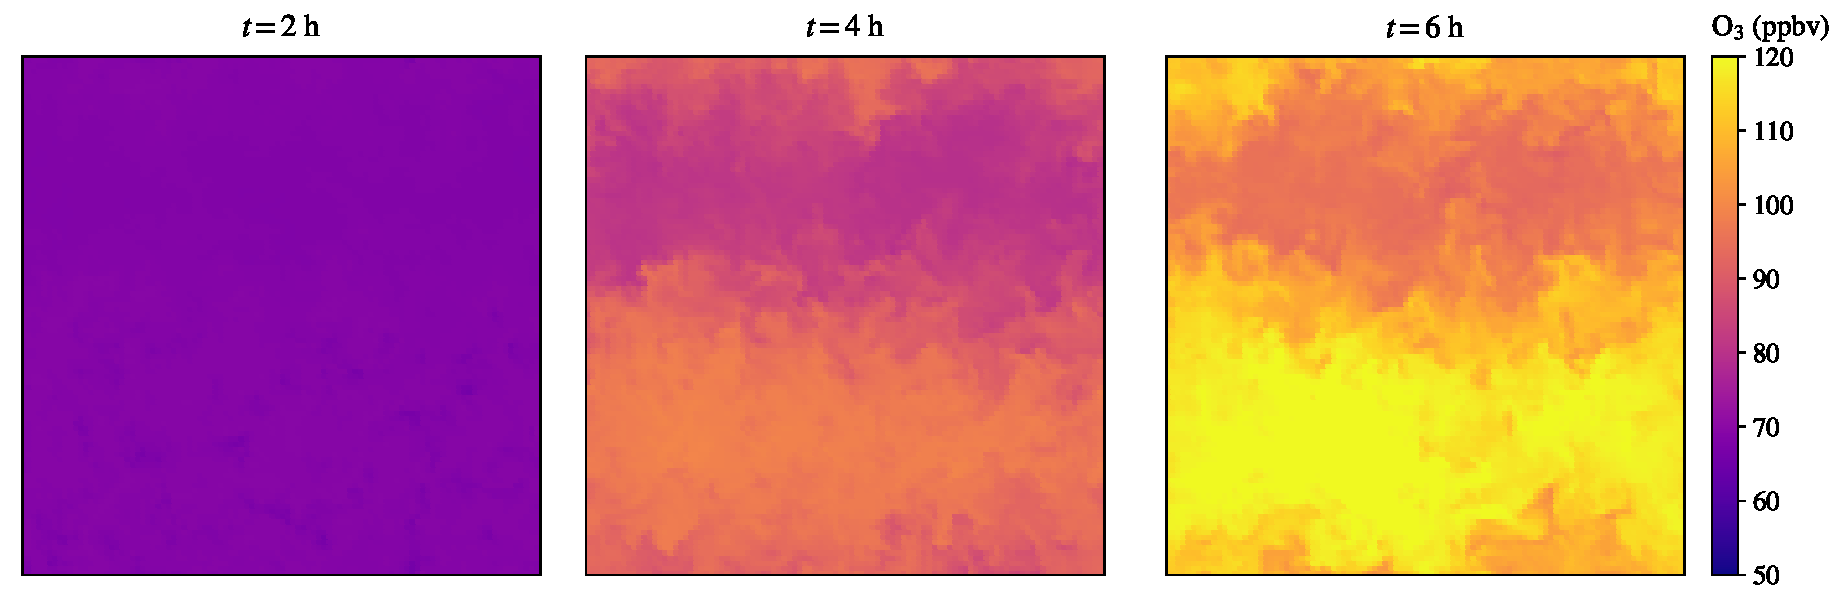
\includegraphics[width=\textwidth]{figures/chapter4/o3-crosssec-fx1fy0-z25.pdf}
    \caption{Ozone cross sections in the x-y plane at 2 hour intervals in the middle of the PBL ($z\sim500$ \si{m}) for emissions scenario 1.}
    \label{fig:o3-crosssec-s1}
  \end{subfigure}
     \vspace*{5mm} 
  \begin{subfigure}
    \centering
    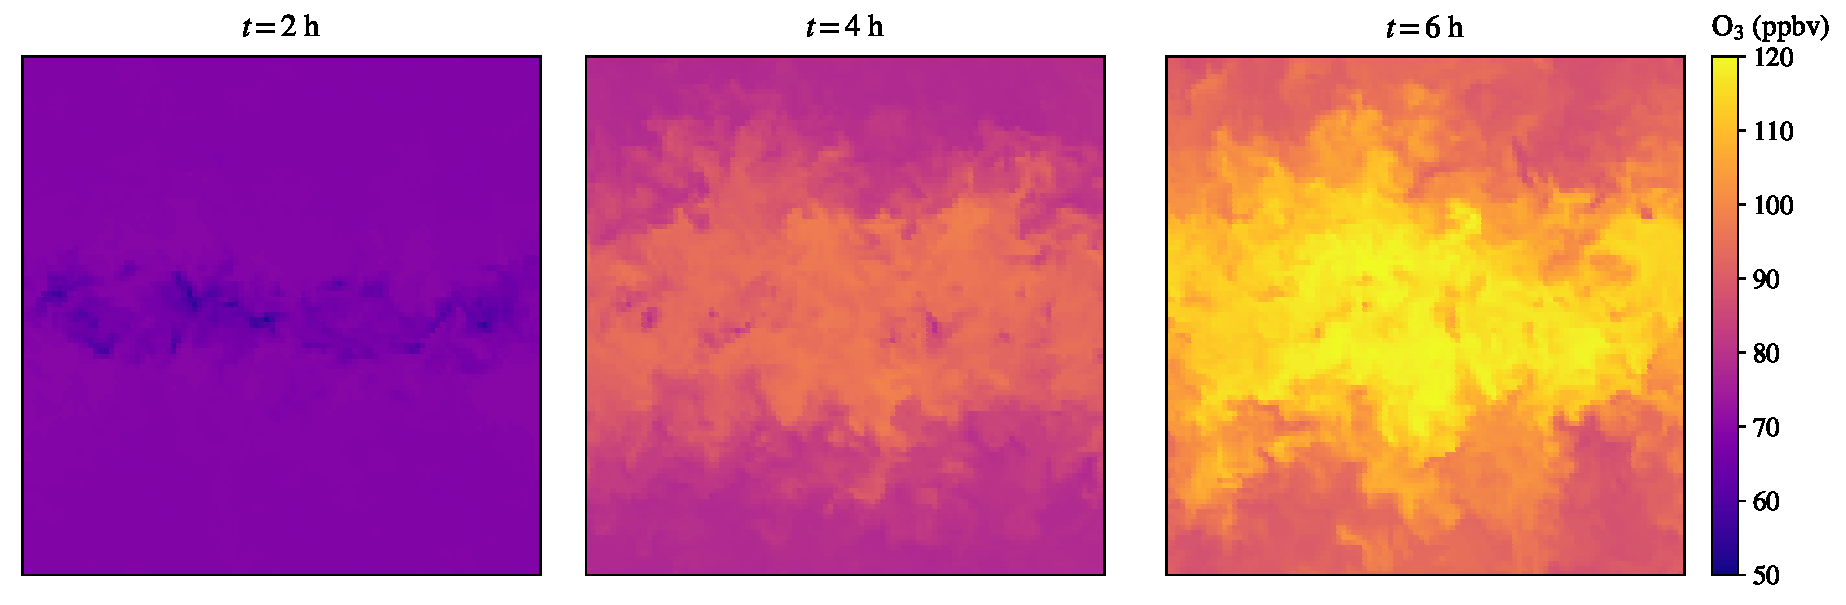
\includegraphics[width=\textwidth]{figures/chapter4/o3-crosssec-road-10x-z25.pdf}
    \caption{Ozone cross sections in the x-y plane at 2 hour intervals in the middle of the PBL ($z\sim500$ \si{m}) for emissions scenario 2.}
    \label{fig:o3-crosssec-s2}
  \end{subfigure}
   \vspace*{5mm} 
  \begin{subfigure}
    \centering
    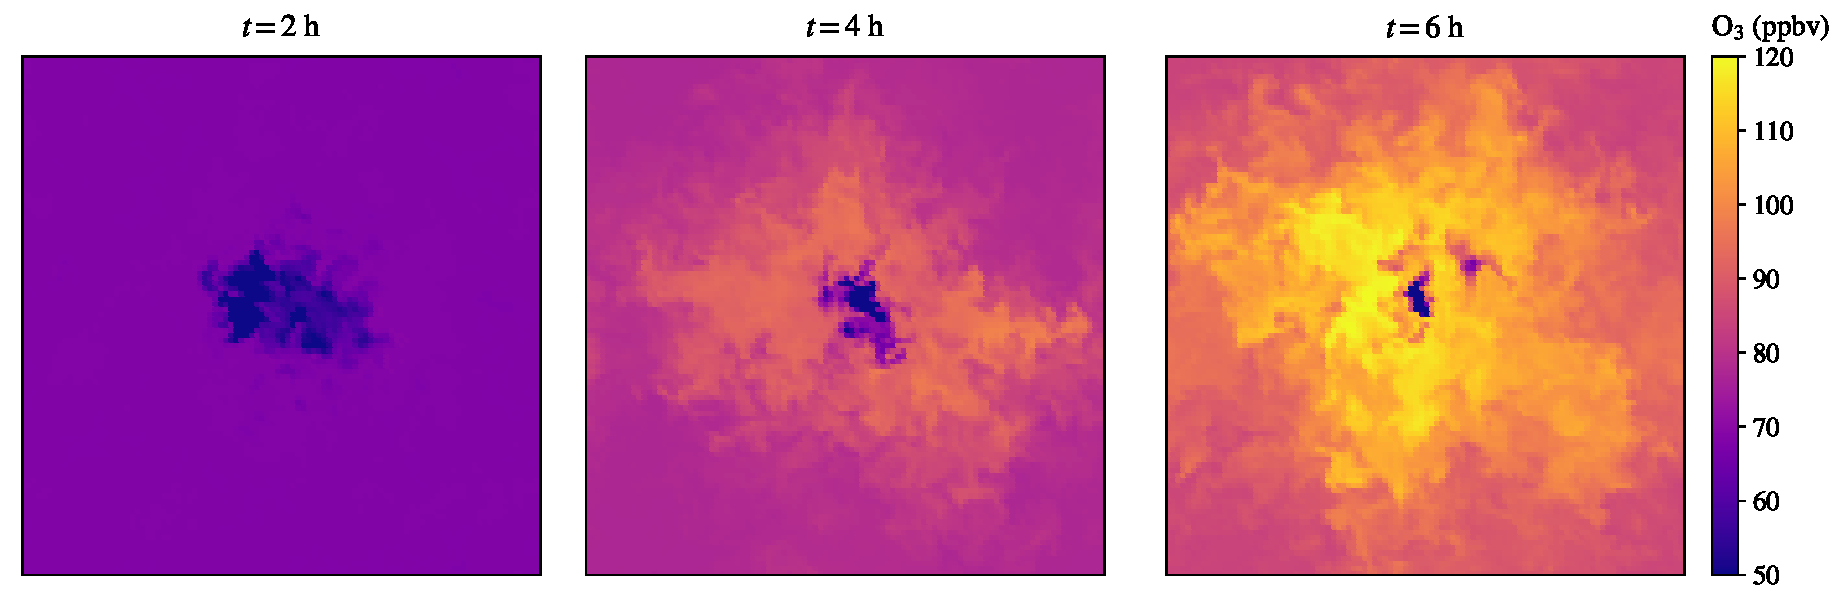
\includegraphics[width=\textwidth]{figures/chapter4/o3-crosssec-point-source-1x1-z25.pdf}
    \caption{Ozone cross sections in the x-y plane at 2 hour intervals in the middle of the PBL ($z\sim500$ \si{m}) for emissions scenario 3.}
    \label{fig:o3-crosssec-s3}
  \end{subfigure}
\end{figure}


%\subsection{Segregation intensity}
\subsection{Spatio-temporal trends in ozone and its precursors}

\begin{figure}[h]
    \centering
    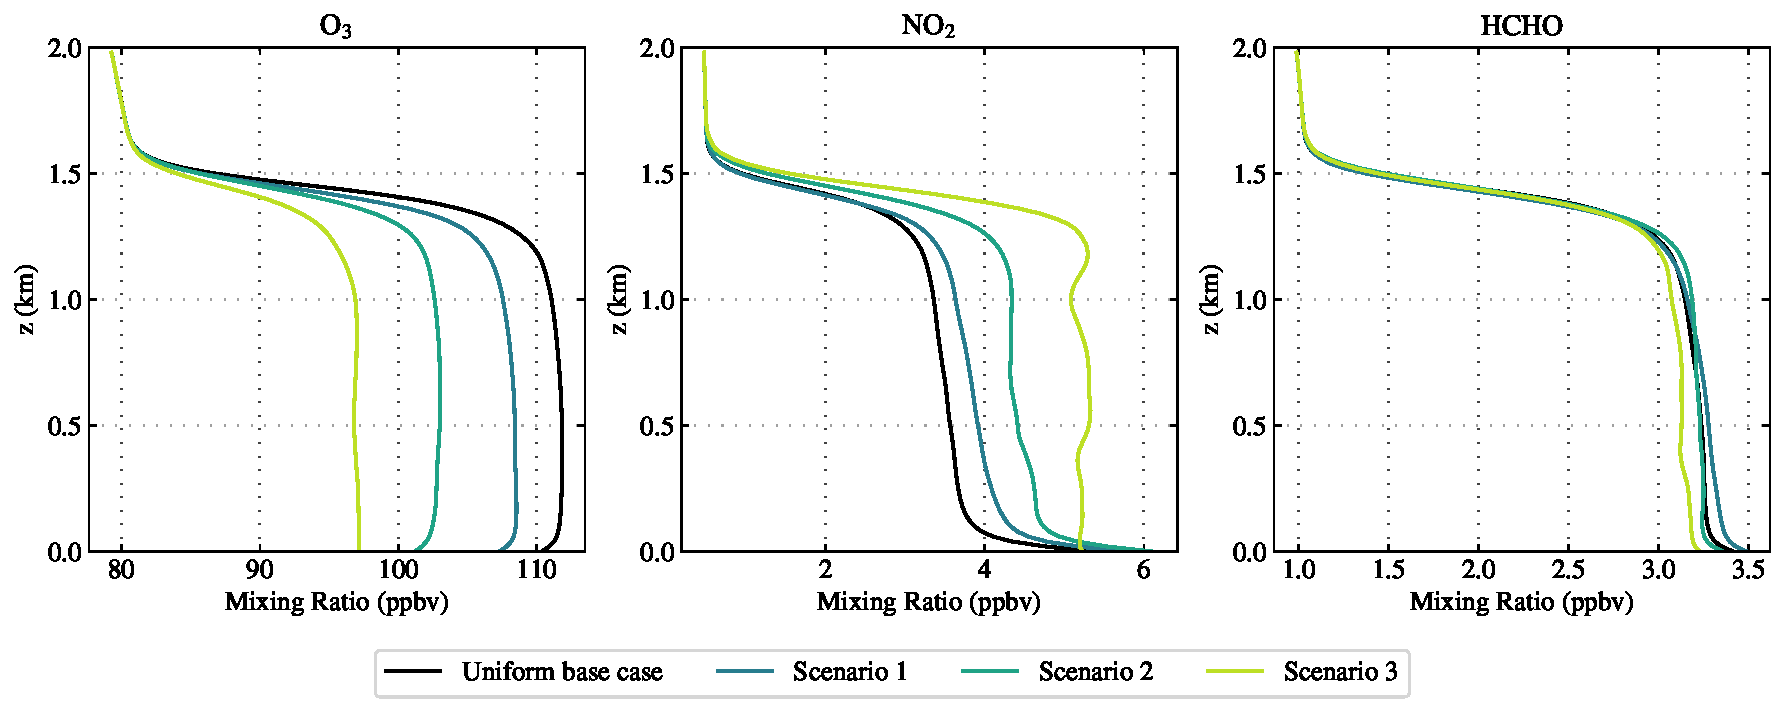
\includegraphics[width=\textwidth]{figures/chapter4/vertical-profiles-time36.pdf}
    \caption{}
    \label{fig:vertical-profiles-o3-nox-hcho}
  \end{figure}

\begin{figure}[h]
    \centering
    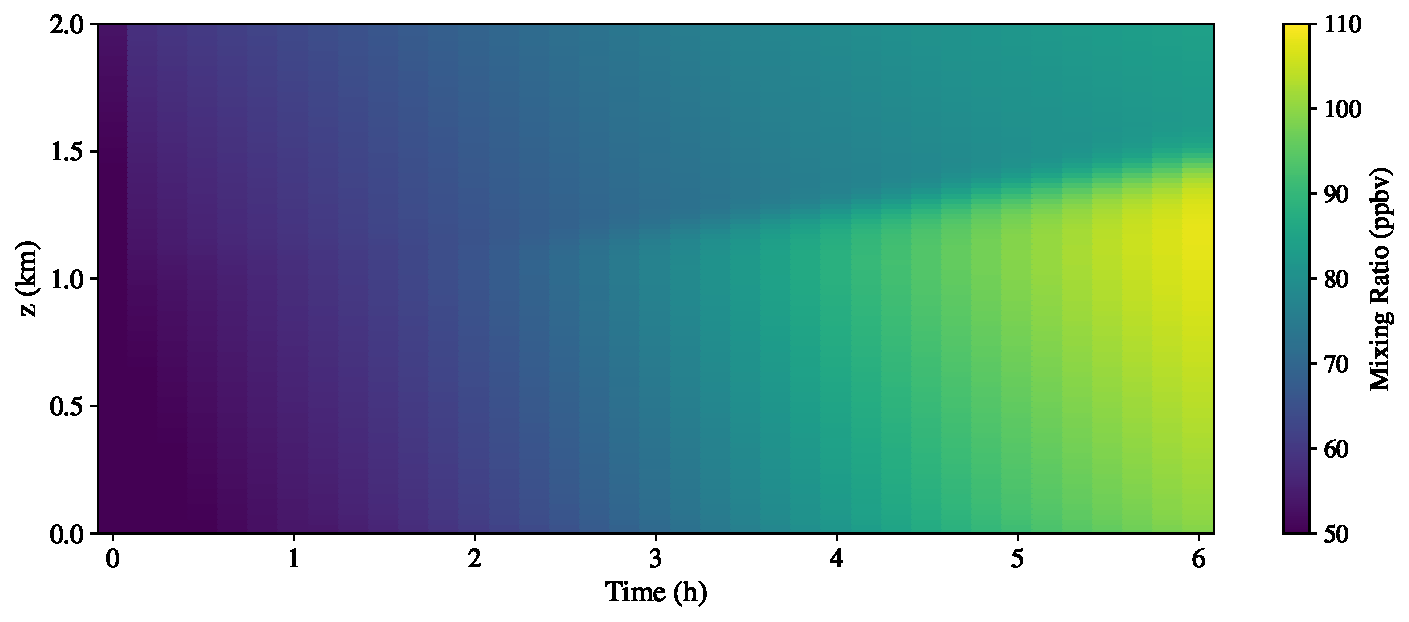
\includegraphics[width=\textwidth]{figures/chapter4/height-time-o3-uniform-basecase.pdf}
    \caption{Ozone concentration height time plot for the uniform base case.}
    %\label{fig:aero_ic_dist}
  \end{figure}
  
\begin{figure}[h]
  \centering
  \begin{subfigure}
    \centering
    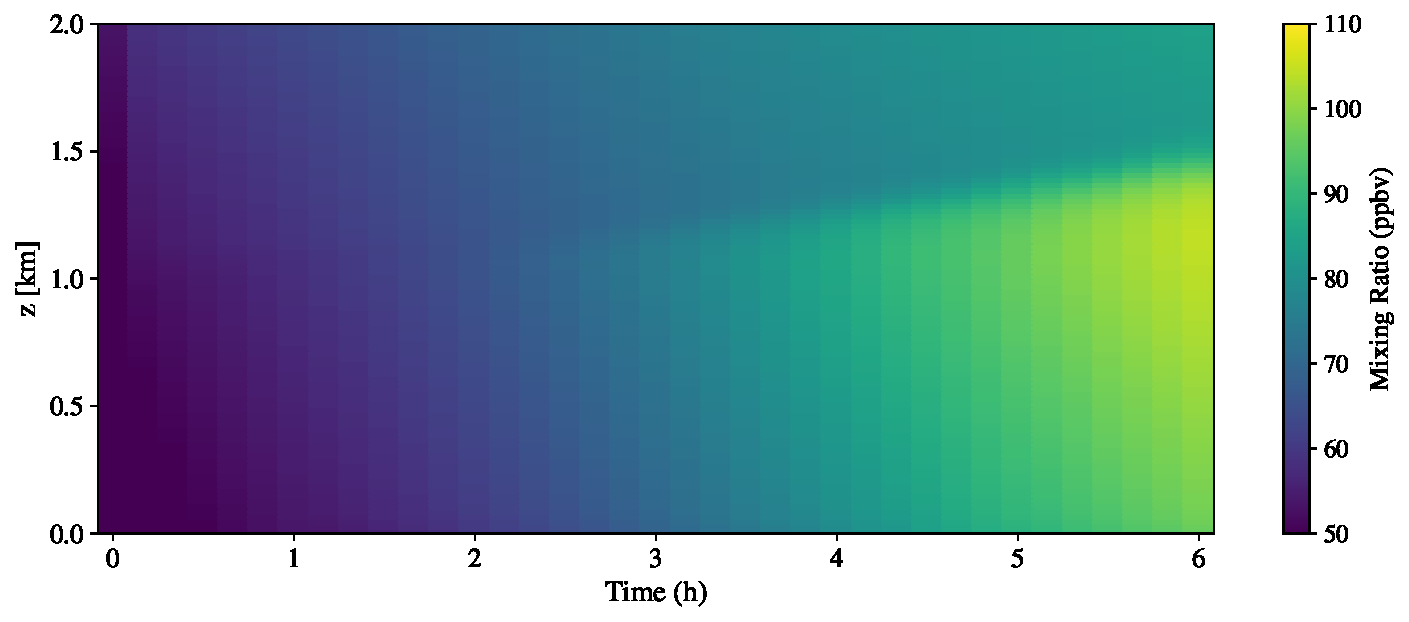
\includegraphics[width=.8\textwidth]{figures/chapter4/height-time-o3-fx1fy0.pdf}
    \caption{Ozone concentration height time plot for emissions scenario 1.}
    %\label{fig:aero_emiss_dist}
  \end{subfigure}
     \vspace*{5mm} 
  \begin{subfigure}
    \centering
    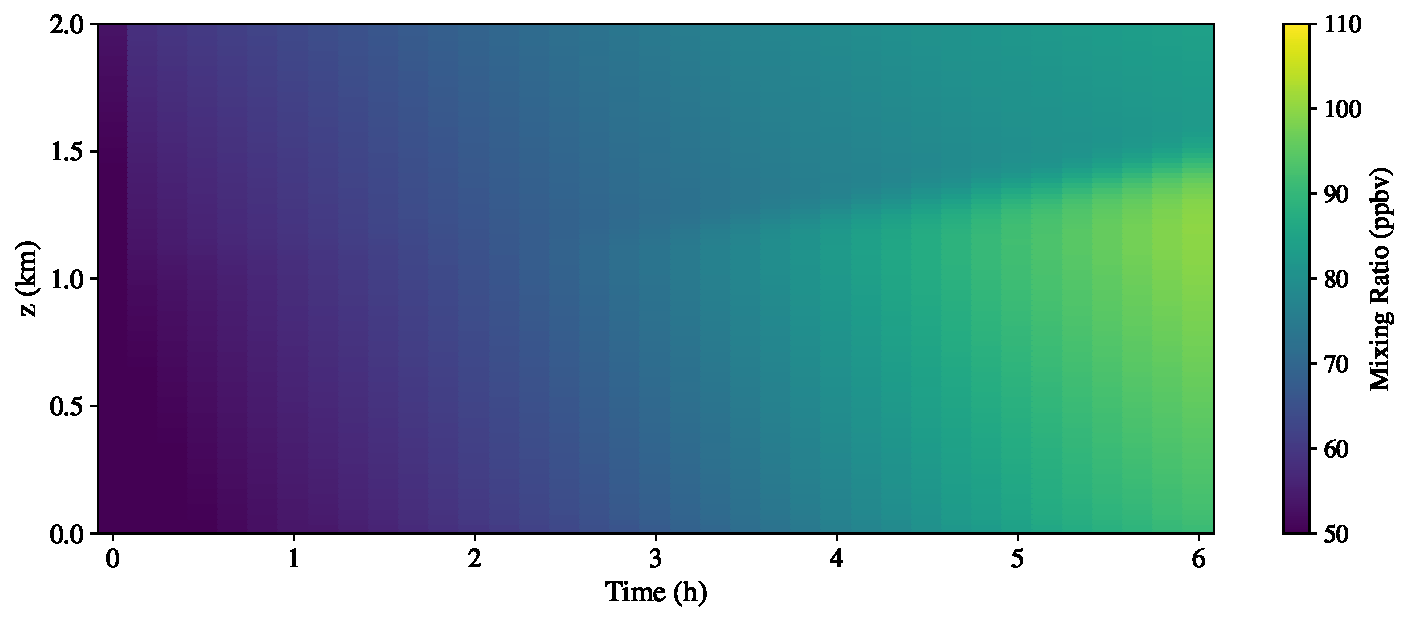
\includegraphics[width=.8\textwidth]{figures/chapter4/height-time-o3-road-10x.pdf}
    \caption{Ozone concentration height time plot for emissions scenario 2.}
    %\label{fig:aero_emiss_dist}
  \end{subfigure}
   \vspace*{5mm} 
  \begin{subfigure}
    \centering
    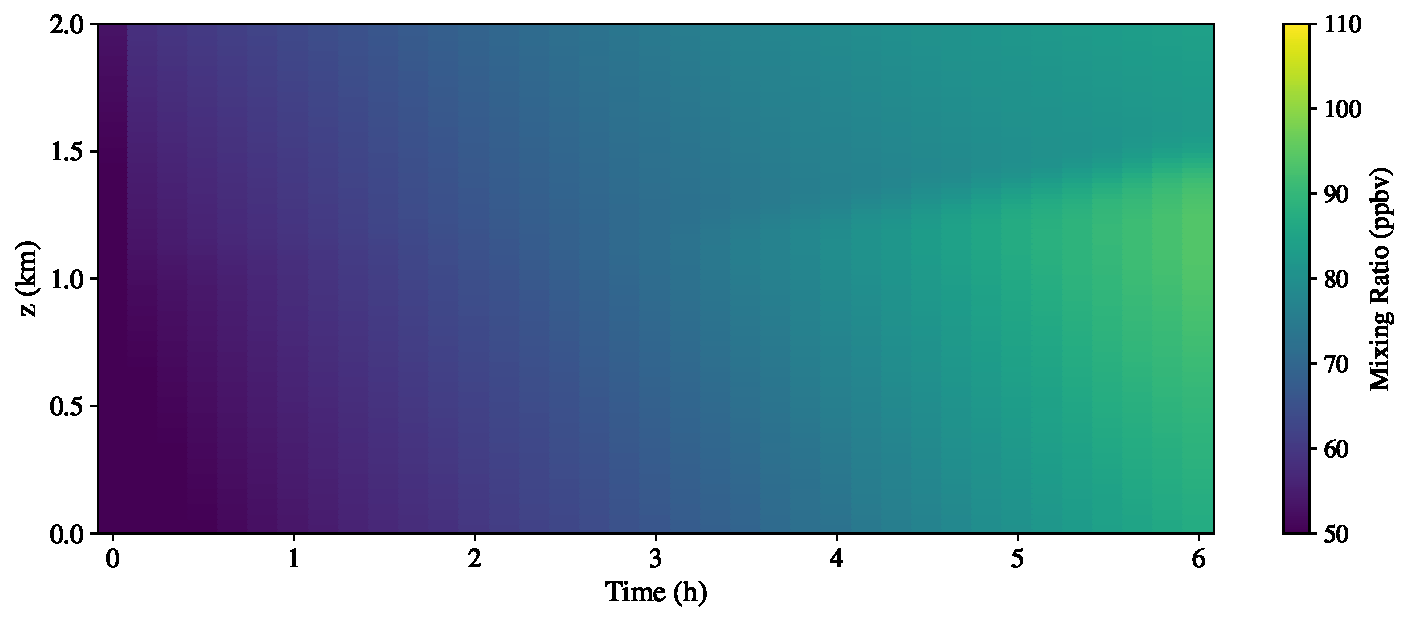
\includegraphics[width=.8\textwidth]{figures/chapter4/height-time-o3-point-source-1x1.pdf}
    \caption{Ozone concentration height time plot for emissions scenario 3.}
    %\label{fig:aero_emiss_dist}
  \end{subfigure}
\end{figure}

\begin{figure}[h]
  \centering
  \begin{subfigure}
    \centering
    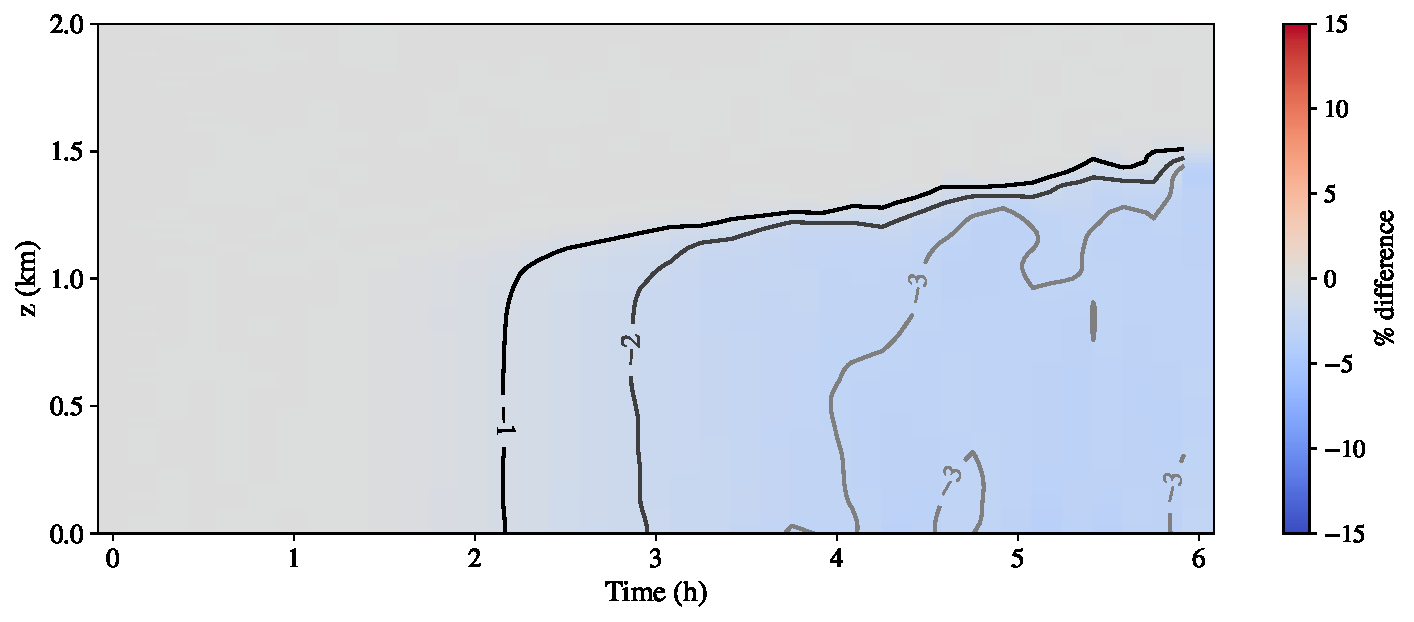
\includegraphics[width=.8\textwidth]{figures/chapter4/height-time-pdiff-o3-fx1fy0.pdf}
    \caption{Height-time plot of ozone percent difference for emissions scenario 1.}
    %\label{fig:aero_emiss_dist}
  \end{subfigure}
     \vspace*{5mm} 
  \begin{subfigure}
    \centering
    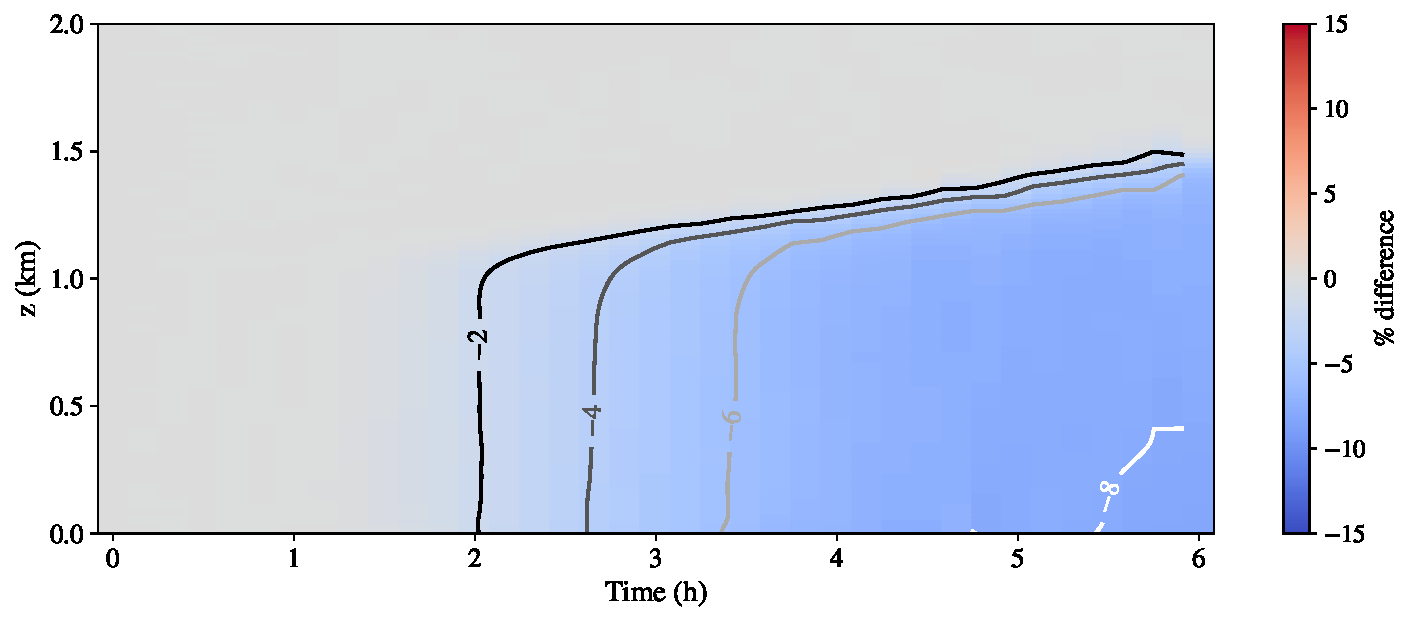
\includegraphics[width=.8\textwidth]{figures/chapter4/height-time-pdiff-o3-road-10x.pdf}
    \caption{Height-time plot of ozone percent difference for emissions scenario 2.}
    %\label{fig:aero_emiss_dist}
  \end{subfigure}
   \vspace*{5mm} 
  \begin{subfigure}
    \centering
    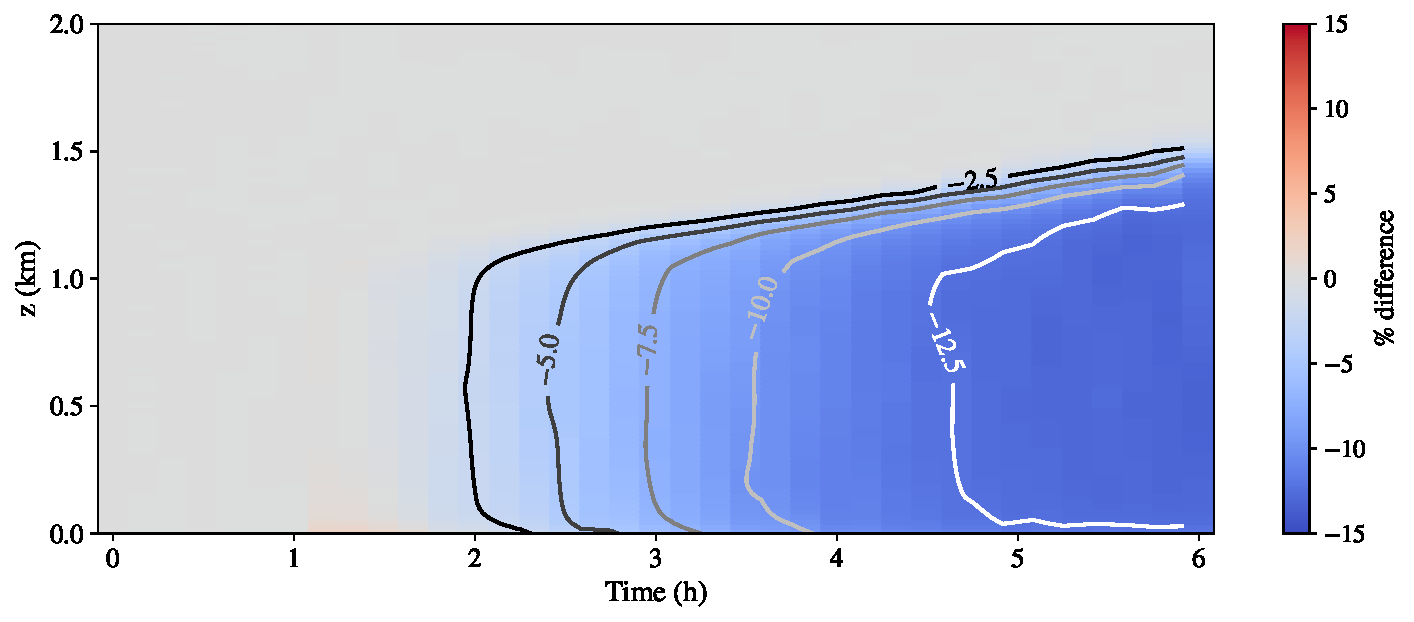
\includegraphics[width=.8\textwidth]{figures/chapter4/height-time-pdiff-o3-point-source-1x1.pdf}
    \caption{Height-time plot of ozone percent difference for emissions scenario 3.}
    %\label{fig:aero_emiss_dist}
  \end{subfigure}
\end{figure}

\subsection{Spatial heterogeneity of ozone and its precursors}

\begin{figure}[h]
  \centering
  \begin{subfigure}
    \centering
    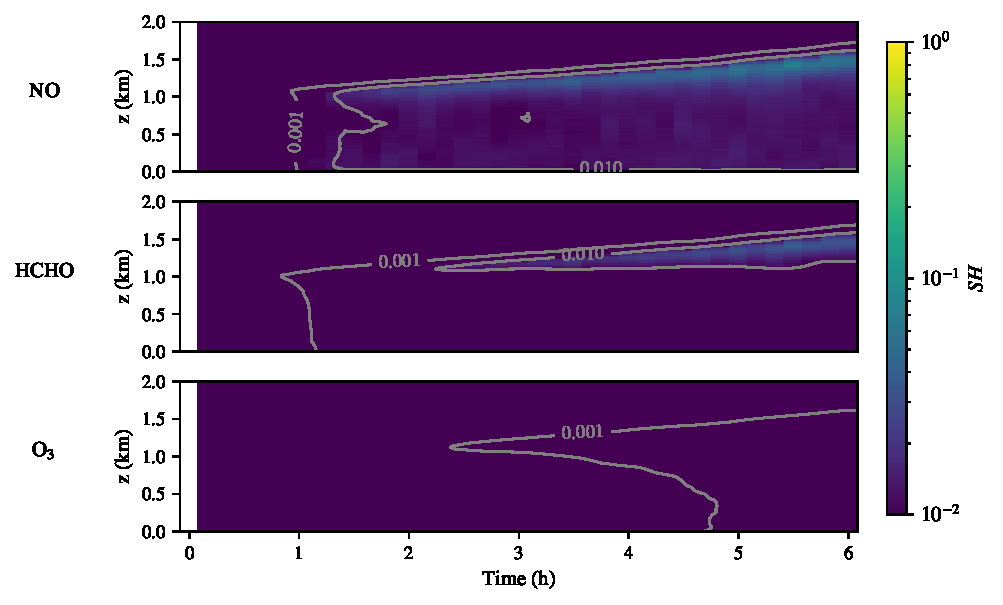
\includegraphics[width=.97\textwidth]{figures/chapter4/height-time-nsh-multivar-uniform-basecase.pdf}
    \caption{Height-time plot of field $SH$ for O$_3$, NO$_x$, and HCHO in the uniform base case. $SH$ value contours are shown in grayscale for each subplot.}
    %\label{fig:aero_emiss_dist}
  \end{subfigure}
     \vspace*{2mm} 
  \begin{subfigure}
    \centering
    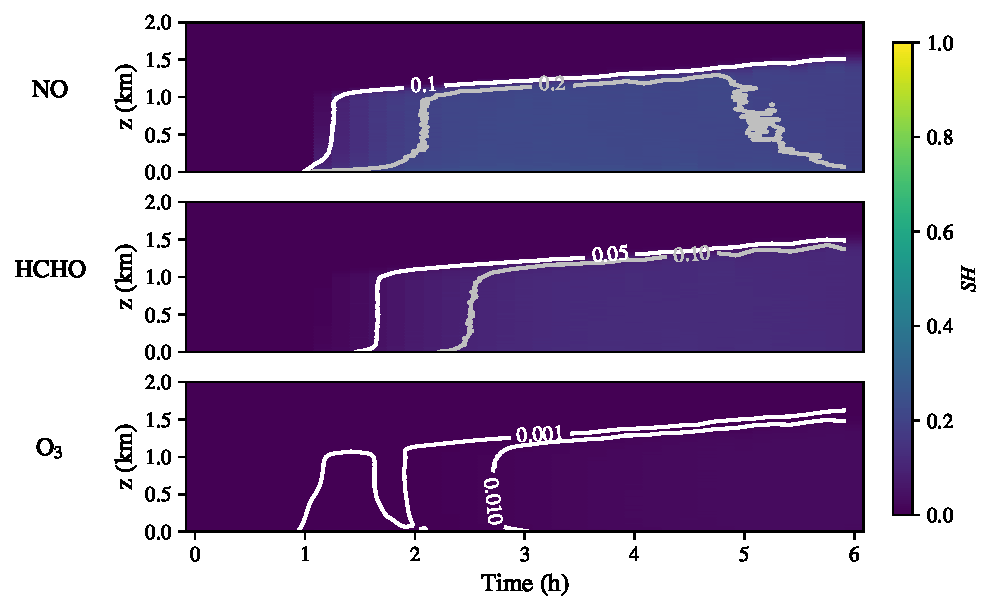
\includegraphics[width=.97\textwidth]{figures/chapter4/height-time-nsh-multivar-fx1fy0.pdf}
    \caption{Height-time plot of field $SH$ for O$_3$, NO$_x$, and HCHO in emissions scenario 1. $SH$ value contours are shown in grayscale for each subplot.}
    %\label{fig:aero_emiss_dist}
  \end{subfigure}
 \end{figure}

\begin{figure}[h]
  \centering
  \begin{subfigure}
    \centering
    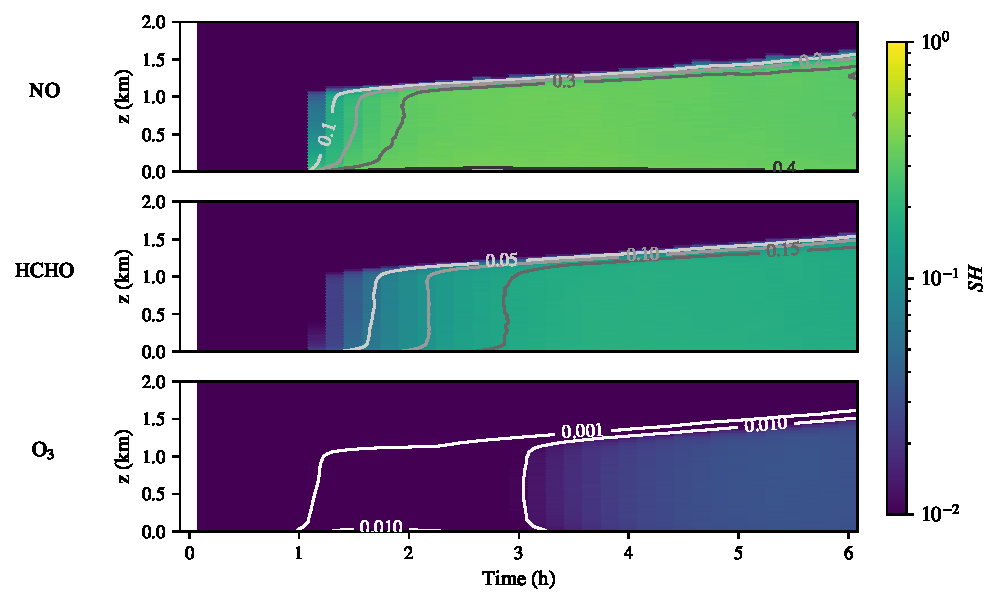
\includegraphics[width=.97\textwidth]{figures/chapter4/height-time-nsh-multivar-road-10x.pdf}
    \caption{Height-time plot of field $SH$ for O$_3$, NO$_x$, and HCHO in emissions scenario 2. $SH$ value contours are shown in grayscale for each subplot.}
    %\label{fig:aero_emiss_dist}
  \end{subfigure}
     \vspace*{2mm} 
  \begin{subfigure}
    \centering
    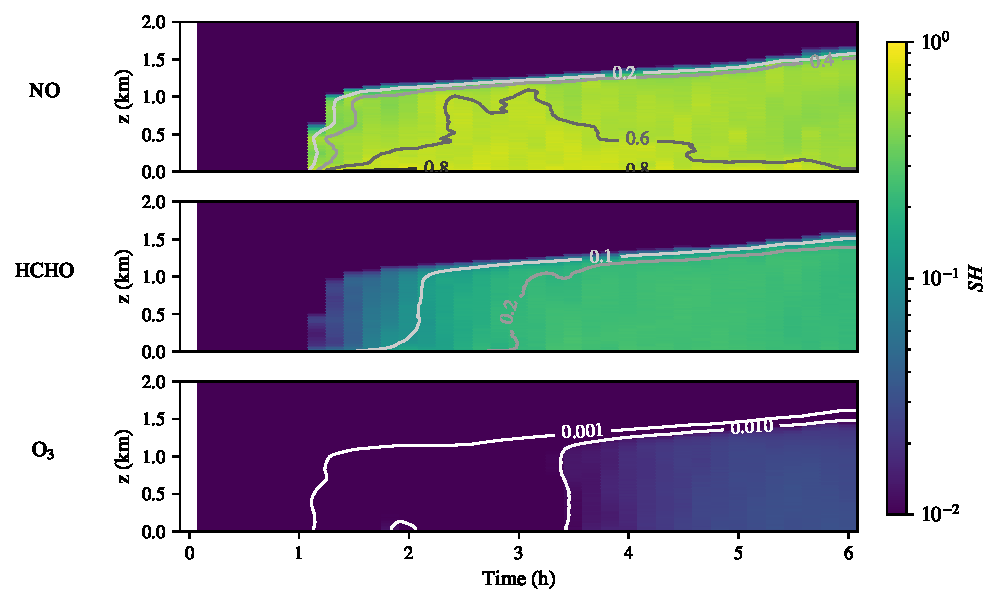
\includegraphics[width=.97\textwidth]{figures/chapter4/height-time-nsh-multivar-point-source-1x1.pdf}
    \caption{Height-time plot of field $SH$ for O$_3$, NO$_x$, and HCHO in emissions scenario 3. $SH$ value contours are shown in grayscale for each subplot.}
    %\label{fig:aero_emiss_dist}
  \end{subfigure}
 \end{figure}



\subsection{Structural uncertainty in ozone production}

%\begin{figure}[h]
%    \centering
%    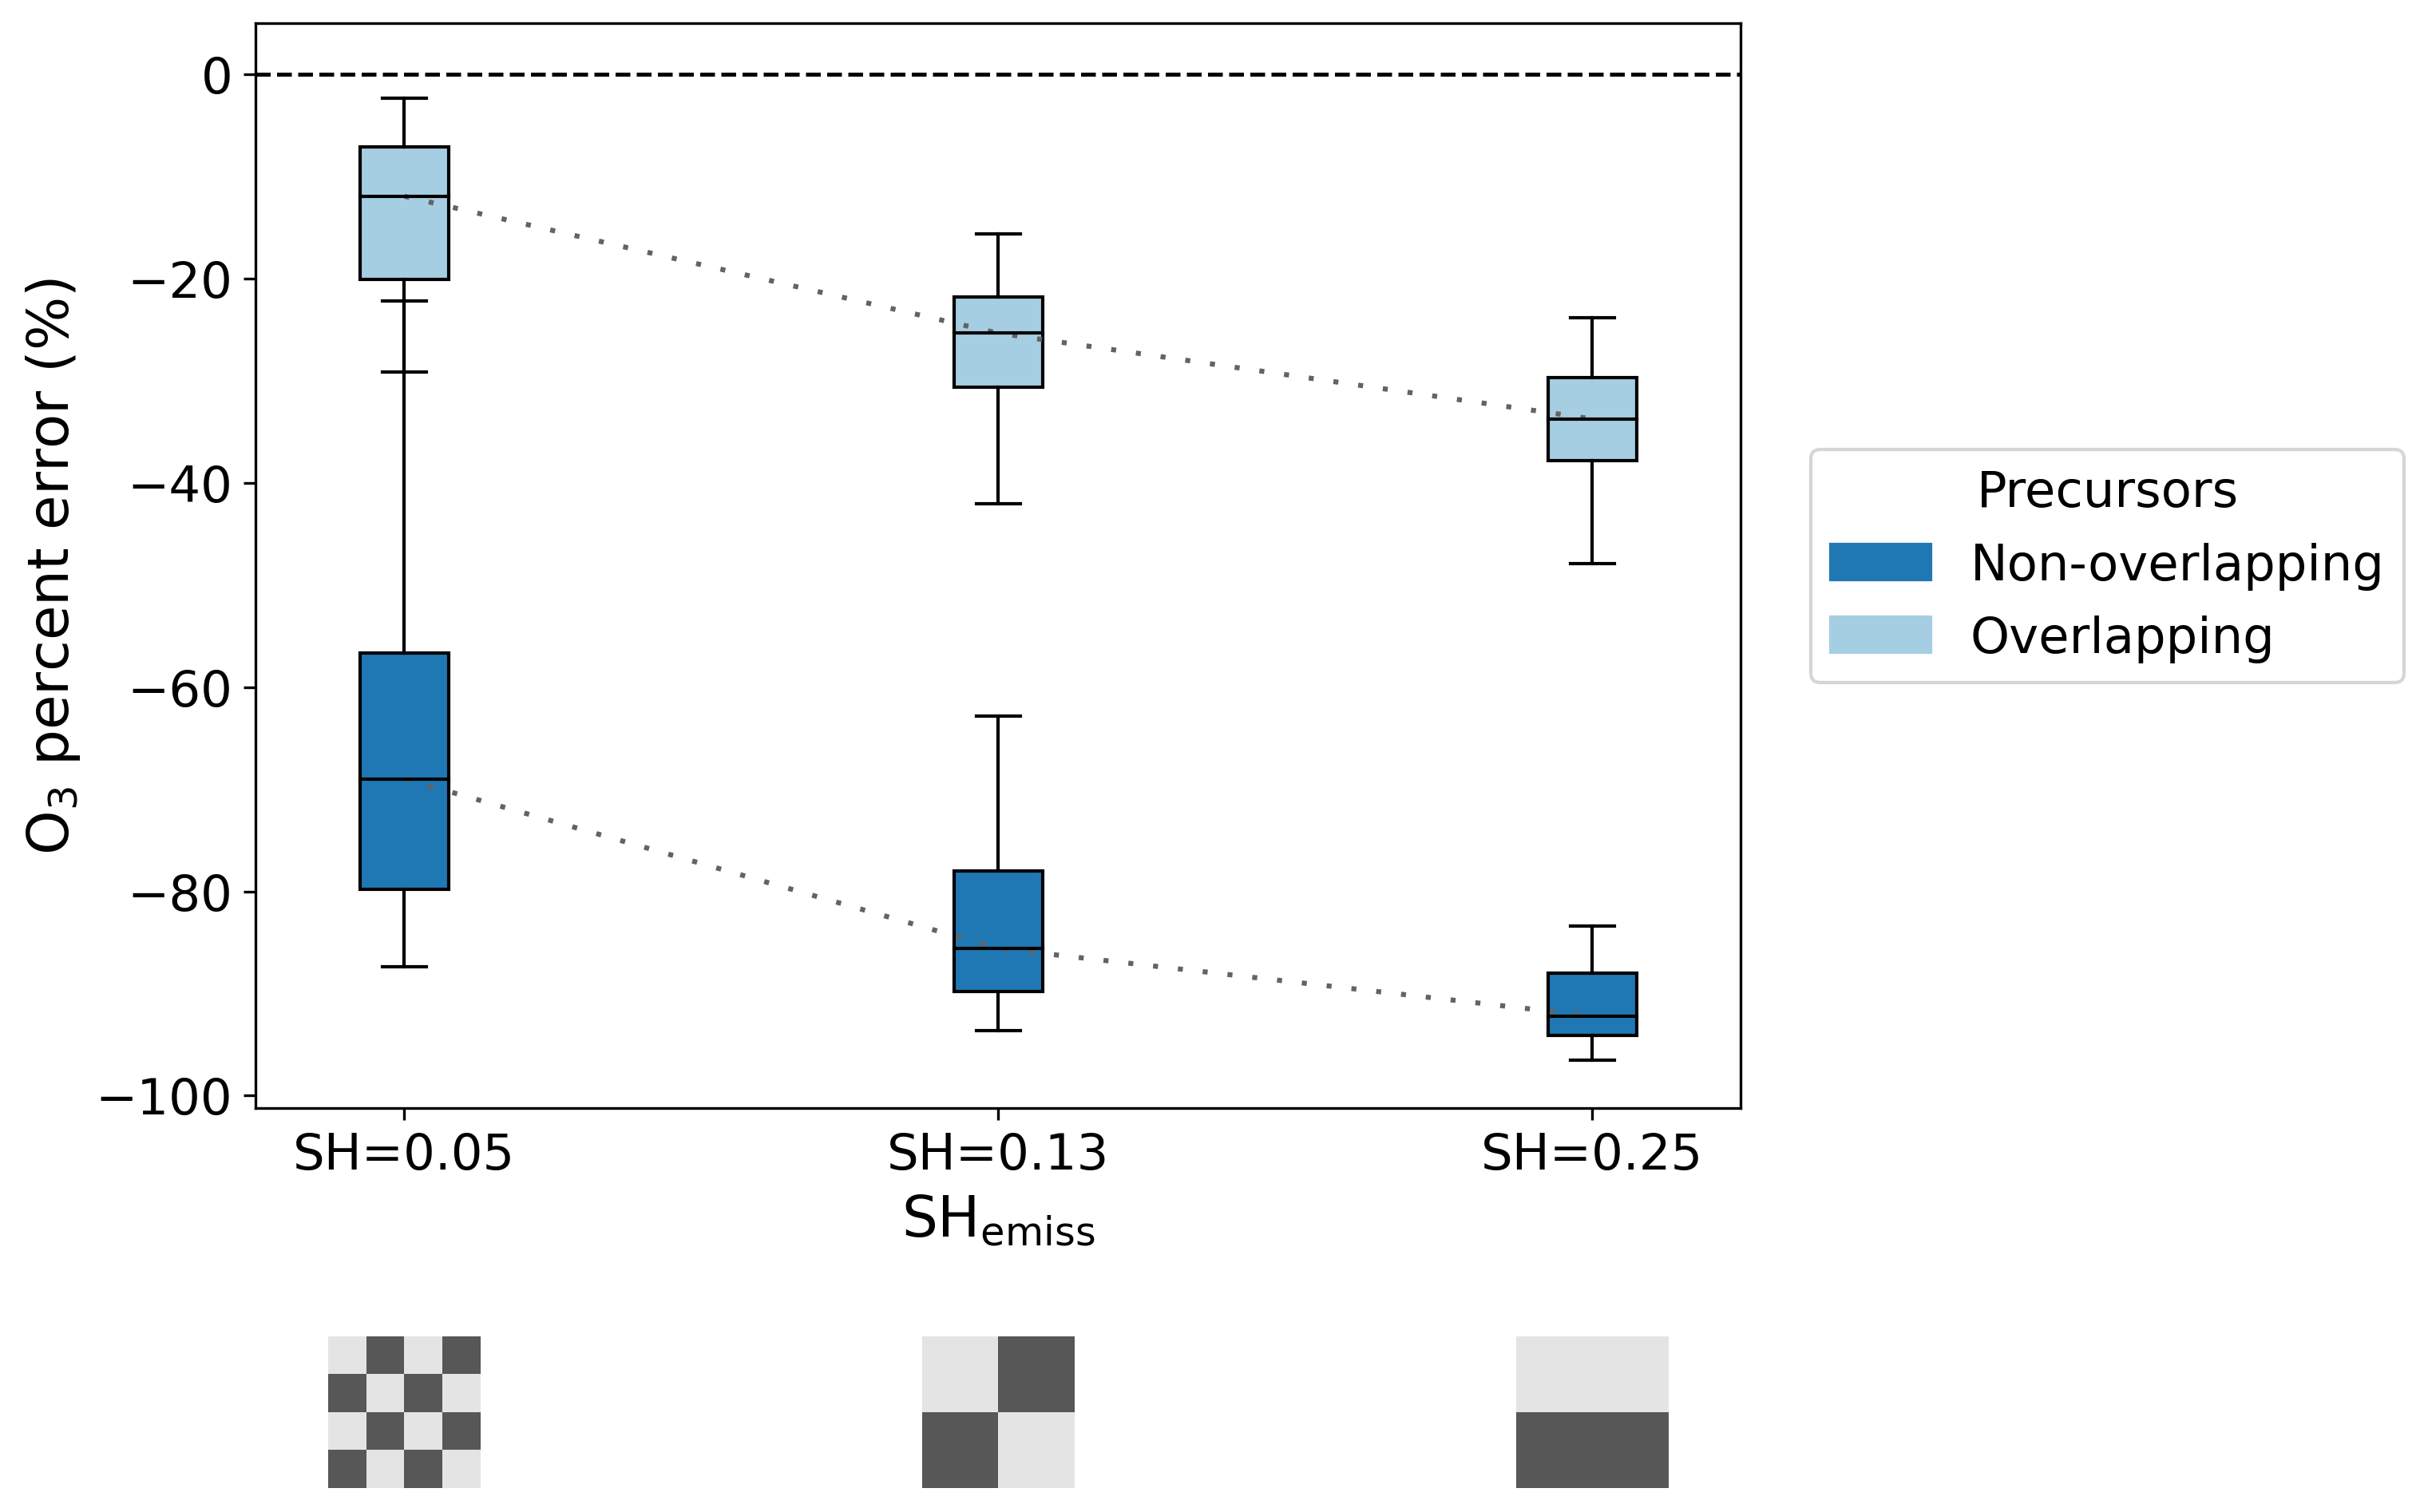
\includegraphics[width=\textwidth]{figures/O3-percent-err-vs-emiss-SH.png}
%    \caption{\hl{Via ARM poster:} Deviation of ozone concentration from case with uniform NOx and VOC emissions. Larger SH in emissions and overlapping emissions lead to larger deviations.}
    %\label{fig:aero_ic_dist}
%  \end{figure}
  
\section{Discussion}

\hl{This either goes here or in the introduction..}
\begin{itemize}
\item Worth noting at some point past studies that have evaluated the production of ozone in LES as well as some studies that investigate the impacts of spatial het. on ozone production (Initial studies investigated idealized interactions between turbulence and ozone chemistry in the PBL, more recent studies have branched into region-specific studies to investigate impacts of spatially heterogeneous emissions and turbulence-chemistry interactions on local ozone production).
\begin{itemize}
\item \cite{schumann_large-eddy_1989} Idealized LES of boundary layer - investigate binary reactions (such as those typical of ozone production) with varying reaction rates. For rates typical of ozone-nox reactions, the mechanism is significantly impacted by turbulence.
\item \cite{sykes_large-eddy_1992} Idealized LES of boundary layer - investigate turbulence chemistry interactions on ozone chemistry, particularly focused on the removal mechanism oxidizing NO to NO2 + O2. Find that the production rate of NO2 is highly dependent on the turbulent mixing of the plume. They show that the turbulence segregation coefficient can be approximated as uniform in a emitted plume. 
%\item \cite{krol_effects_2000} Maybe?
\item \cite{auger_chemical_2007} (seems very similar to what I am doing here) LES of PBL over 10x10 km domain. Indicate that segregation is strongest in the first two hours - after 3 hours segregation is largely reduced due to efficient mixing in the PBL. 
\item \cite{zhong_modelling_2015} Similar to Zhong et al 2017, find that ozone production rate is reduced due to incomplete mixing.
\item \cite{zhong_large_2017} LES study of O3-NOx-VOC chemistry in urban street canyons characterized by high spatial variability in concentration gradients. NOx and HOx radicals were consumed to produce NO2 and O3. Segregation effect due to incomplete mixing reduces the production of NO2. 
\item \cite{wang_impact_2021}
\item \cite{wang_segregation_2022} Similar to wang 2023
\item \cite{wang_coupled_2023} Use of LES (WRF-Chem LES \hl{what chem mechanism?}) for urban (Hong Kong) emissions compared against mesoscale simulations, show that NOx is underestimated and O3 overestimated in mesoscale simulations when compared to LES, attributed to the higher spatial resolution of emissions and explicitly resolving turbulent transport.
\end{itemize} 
\end{itemize}




